% !TEX options=--shell-escape

%%%%%%%%%%%%%%%%%%%%%%%%%%%%%%%%%%%%%%%%%%%%%%%%%%%%%%%
% MatPlotLib and Random Cheat Sheet
%
% Edited by Michelle Cristina de Sousa Baltazar
%
% http://matplotlib.org/api/pyplot_summary.html
% http://matplotlib.org/users/pyplot_tutorial.html
%
%%%%%%%%%%%%%%%%%%%%%%%%%%%%%%%%%%%%%%%%%%%%%%%%%%%%%%%

\documentclass{article}
\usepackage[a4paper, landscape]{geometry}
\usepackage{url}
\usepackage{multicol}
\usepackage{amsmath}
\usepackage{amsfonts}
\usepackage{tikz}
\usetikzlibrary{decorations.pathmorphing}
\usepackage{amsmath,amssymb}
\usepackage{graphicx}

\usepackage{colortbl}
\usepackage{xcolor}
\usepackage{mathtools}
\usepackage{amsmath,amssymb}
\usepackage{enumitem}
\usepackage{bold-extra}
\usepackage{changepage}

\usepackage{minted}
\usemintedstyle{trac}
\newminted{cpp}{autogobble,escapeinside=@@,fontsize=\footnotesize}
\newminted{python}{autogobble,escapeinside=@@,fontsize=\footnotesize}
\newminted{sh}{autogobble,escapeinside=@@,fontsize=\footnotesize}

\definecolor{green}{rgb}{0.01,0.4,0.01}
\definecolor{red}{rgb}{0.4,0.01,0.01}

\title{CS328 Python Cheat Sheet}
\usepackage[brazilian]{babel}
\usepackage[utf8]{inputenc}

\advance\topmargin-.8in
\advance\textheight3in
\advance\textwidth3in
\advance\oddsidemargin-1.5in
\advance\evensidemargin-1.5in
\parindent0pt
\parskip2pt
\setlength{\footskip}{50px}
\newcommand{\hr}{\centerline{\rule{3.5in}{1pt}}}
%\colorbox[HTML]{e4e4e4}{\makebox[\textwidth-2\fboxsep][l]{texto}

\renewcommand{\familydefault}{\sfdefault}

\begin{document}

\tikzstyle{mybox} = [draw=black, fill=white, very thick,
    rectangle, rounded corners, inner sep=10pt, inner ysep=10pt]
\tikzstyle{fancytitle} =[fill=green, text=white, font=\bfseries]

\begin{multicols*}{3}
%
\begin{center}{\LARGE{\textbf{Python 3 Cheat Sheet}}}\par
{\large EPFL CS 328\\ Numerical Methods for Visual Computing}\\
{\footnotesize (Version 1)}
\end{center}

\vspace*{-0.3cm}

%============ BASICS ==============================================

%------------ Basic data types and introspection ---------------
\begin{tikzpicture}
\node [mybox] (box){%
	\begin{minipage}{0.3\textwidth}
	Basic native data types:
	\begin{center}\small{\begin{tabular}{lp{4cm} l}
		\hline
		Integer \qquad\qquad\qquad\enspace&
		\begin{minipage}[t]{\textwidth}
		\begin{pythoncode}
		i = 42
		\end{pythoncode}
		\end{minipage}
		\\ \hline
		Float &
		\begin{minipage}[t]{\textwidth}
		\begin{pythoncode}
		3.14159
		\end{pythoncode}
		\end{minipage}
		\\ \hline
		Complex number &
		\begin{minipage}[t]{\textwidth}
		\begin{pythoncode}
		2 + 3j
		\end{pythoncode}
		\end{minipage}
		\\ \hline
		Boolean &
		\begin{minipage}[t]{\textwidth}
		\begin{pythoncode}
		b = True
		\end{pythoncode}
		\end{minipage}
		\\ \hline
		String &
		\begin{minipage}[t]{\textwidth}
		\begin{pythoncode}
		s = 'spam'
		\end{pythoncode}
		\end{minipage}
		\\ \hline
		None type. &
		\begin{minipage}[t]{\textwidth}
		\begin{pythoncode}
		n = None
		\end{pythoncode}
		\end{minipage}
		\\ \hline
		\end{tabular}}\end{center}
	
	Introspection functions:
	\begin{center}\small{\begin{tabular}{lp{4cm} l}
		\hline
		Type of an object &
		\begin{minipage}[t]{\textwidth}
		\begin{pythoncode}
		type(var)
		\end{pythoncode}
		\end{minipage}
		\\ \hline
		Built-in system help &
		\begin{minipage}[t]{\textwidth}
		\begin{pythoncode}
		help(var)
		\end{pythoncode}
		\end{minipage}
		\\ \hline
		Lists objetc's attributes &
		\begin{minipage}[t]{\textwidth}
		\begin{pythoncode}
		dir(var)
		\end{pythoncode}
		\end{minipage}
		\\ \hline
		Class membership test &
		\begin{minipage}[t]{\textwidth}
		\begin{pythoncode}
		isinstance(var, class)
		\end{pythoncode}
		\end{minipage}
		\\ \hline
		\end{tabular}}\end{center}
	\end{minipage}
};
\node[fancytitle, right=10pt] at (box.north west) {Basic data yypes and introspection};
\end{tikzpicture}

%------------ Operators ---------------
\begin{tikzpicture}
\node [mybox] (box){%
    \begin{minipage}{0.3\textwidth}
            Arithmetic operators:
            \begin{center}\small{\begin{tabular}{lp{4cm} l}
                \hline
                Addition &
                \begin{minipage}[t]{\textwidth}
                \begin{pythoncode}
                    x + y
                \end{pythoncode}
                \end{minipage}
                \\ \hline
                Subtraction &
                \begin{minipage}[t]{\textwidth}
                \begin{pythoncode}
                    x - y
                \end{pythoncode}
                \end{minipage}
                \\ \hline
                Floating point division &
                \begin{minipage}[t]{\textwidth}
                \begin{pythoncode}
                    x / y
                \end{pythoncode}
                \end{minipage}
                \\ \hline
                Integer division &
                \begin{minipage}[t]{\textwidth}
                \begin{pythoncode}
                    x // y
                \end{pythoncode}
                \end{minipage}
                \\ \hline
                Multiplication &
                \begin{minipage}[t]{\textwidth}
                \begin{pythoncode}
                    x * y
                \end{pythoncode}
                \end{minipage}
                \\ \hline
                Exponentiation &
                \begin{minipage}[t]{\textwidth}
                \begin{pythoncode}
                    x ** y
                \end{pythoncode}
                \end{minipage}
                \\ \hline
            \end{tabular}}\end{center}

            Boolean operators:
            \begin{center}\small{\begin{tabular}{lp{4cm} l}
                \hline
                And \qquad\qquad\qquad\enspace\enspace\;\; &
                \begin{minipage}[t]{\textwidth}
                \begin{pythoncode}
                    x and y
                \end{pythoncode}
                \end{minipage}
                \\ \hline
                Or &
                \begin{minipage}[t]{\textwidth}
                \begin{pythoncode}
                    x or y
                \end{pythoncode}
                \end{minipage}
                \\ \hline
                Negation &
                \begin{minipage}[t]{\textwidth}
                \begin{pythoncode}
                    not x
                \end{pythoncode}
                \end{minipage}
                \\ \hline
                Unpacking &
                \begin{minipage}[t]{\textwidth}
                \begin{pythoncode}
                    u, v, w = t
                \end{pythoncode}
                \end{minipage}
                \\ \hline
            \end{tabular}}\end{center}
    \end{minipage}
};
\node[fancytitle, right=10pt] at (box.north west) {Operators};
\end{tikzpicture}

%------------ Printing ---------------
\begin{tikzpicture}
\node [mybox] (box){%
    \begin{minipage}{0.3\textwidth}
            Simple print statement:
            \begin{adjustwidth}{0.5cm}{}
            \begin{pythoncode}
                print("Hello!")
            \end{pythoncode}
            \end{adjustwidth}

            String formatting:
            \begin{center}\small{\begin{tabular}{lp{4cm} l}
                \hline
                Integers &
                \begin{minipage}[t]{\textwidth}
                \begin{pythoncode}
                    "int: %d" % 5
                \end{pythoncode}
                \end{minipage}
                \\ \hline
                Floats &
                \begin{minipage}[t]{\textwidth}
                \begin{pythoncode}
                    "float: %f" % 3.14
                \end{pythoncode}
                \end{minipage}
                \\ \hline
                Strings &
                \begin{minipage}[t]{\textwidth}
                \begin{pythoncode}
                    "str: %s" % "foo"
                \end{pythoncode}
                \end{minipage}
                \\ \hline
                Multiple values via tuples &
                \begin{minipage}[t]{\textwidth}
                \begin{pythoncode}
                    "two ints: %d %d" % (1, 2)
                \end{pythoncode}
                \end{minipage}
                \\ \hline
            \end{tabular}}\end{center}
    \end{minipage}
};
\node[fancytitle, right=10pt] at (box.north west) {Printing and strings};
\end{tikzpicture}


{\LaTeX} template by Michelle Cristina de Sousa Baltazar.

% Start next column
\vfill\null
\columnbreak

%============ ABSTRACT DATATYPES ==================================

%------------ LISTS ---------------
\begin{tikzpicture}
\node [mybox] (box){%
	\begin{minipage}{0.3\textwidth}
	Ordered sequence of elements of arbitrary data types.
	\begin{center}\small{\begin{tabular}{lp{4cm} l}
		\hline
		Create empty &
		\begin{minipage}[t]{\textwidth}
		\begin{pythoncode}
		empty_l = []
		\end{pythoncode}
		\end{minipage}
		\\ \hline
		Create example &
		\begin{minipage}[t]{\textwidth}
		\begin{pythoncode}
		l = ['zero', 1, 2.0, 3 + 0j]
		\end{pythoncode}
		\end{minipage}
		\\ \hline
		Retrieve item (idx from 0) &
		\begin{minipage}[t]{\textwidth}
		\begin{pythoncode}
		d[2]     # Returns 2.0
		\end{pythoncode}
		\end{minipage}
		\\ \hline
		Change item &
		\begin{minipage}[t]{\textwidth}
		\begin{pythoncode}
		l[2] = 'two_point_o' 
		\end{pythoncode}
		\end{minipage}
		\\ \hline
		Query length &
		\begin{minipage}[t]{\textwidth}
		\begin{pythoncode}
		len(l)  # Returns 4
		\end{pythoncode}
		\end{minipage}
		\\ \hline
		Append value to the end &
		\begin{minipage}[t]{\textwidth}
		\begin{pythoncode}
		l.append(4)
		\end{pythoncode}
		\end{minipage}
		\\ \hline
		Extend by another list. &
		\begin{minipage}[t]{\textwidth}
		\begin{pythoncode}
		l.extend([5, 6])
		\end{pythoncode}
		\end{minipage}
		\\ \hline
		\end{tabular}}\end{center}
	
	\vspace*{-0.2cm}
	Looping through all items:
	%
	\begin{adjustwidth}{0.5cm}{}
	\begin{pythoncode}
	for it in l:
	# do something..
	\end{pythoncode}
	\end{adjustwidth}
	%
	%
	\end{minipage}
};
\node[fancytitle, right=10pt] at (box.north west) {Lists};
\end{tikzpicture}

%------------ LISTS - SLICING ---------------
\begin{tikzpicture}
\node [mybox] (box){%
	\begin{minipage}{0.3\textwidth}
	\begin{pythoncode}
		a = ['a', 'b', 'c', 'd', 'e']
	\end{pythoncode}

	\vspace*{-0.3cm}
%	\centering{
%		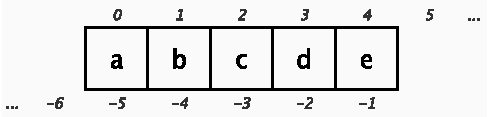
\includegraphics[width=0.7\linewidth]{img/slicing.pdf}
%	}
	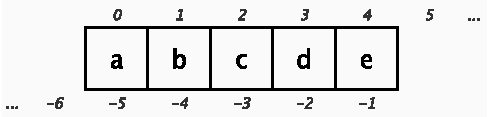
\includegraphics[width=0.7\linewidth]{img/slicing.pdf}
	
	Syntax \texttt{[start:end]} (start - incl., end - excl., step=1)
	
	\begin{center}\small{\begin{tabular}{lp{4cm} l}
		\hline
		Explicit start/end &
		\begin{minipage}[t]{\textwidth}
		\begin{pythoncode}
		a[2:4] # Returns ['c', 'd']
		\end{pythoncode}
		\end{minipage}
		\\ \hline
		Implicit end (incl.) &
		\begin{minipage}[t]{\textwidth}
		\begin{pythoncode}
		a[2:] # Returns ['c', 'd', 'e']
		\end{pythoncode}
		\\ \hline
		Implicit start &
		\begin{minipage}[t]{\textwidth}
		\begin{pythoncode}
		a[:3] # Returns ['a', 'd', 'e']
		\end{pythoncode}
		\\ \hline
		\end{minipage}
		\end{tabular}}\end{center}
	
	Syntax \texttt{[start:end:step]}

	\end{minipage}
};
\node[fancytitle, right=10pt] at (box.north west) {Slicing lists};
\end{tikzpicture}

%------------ DICTIONARIES ---------------
\begin{tikzpicture}
\node [mybox] (box){%
    \begin{minipage}{0.3\textwidth}
        Mapping of key-value pairs.
        \begin{center}\small{\begin{tabular}{lp{5cm} l}
            \hline
            Create empty &
            \begin{minipage}[t]{\textwidth}
            \begin{pythoncode}
                empty_d = {}
            \end{pythoncode}
            \end{minipage}
            \\ \hline
            Create example &
            \begin{minipage}[t]{\textwidth}
            \begin{pythoncode}
                d = {'name': 'Alice', 'age': 25}
            \end{pythoncode}
            \end{minipage}
            \\ \hline
            Retrieve entry &
            \begin{minipage}[t]{\textwidth}
            \begin{pythoncode}
                d['age']     # Returns 25
            \end{pythoncode}
            \end{minipage}
            \\ \hline
            Add / change entry &
            \begin{minipage}[t]{\textwidth}
            \begin{pythoncode}
                d['city'] = 'Lausanne'
            \end{pythoncode}
            \end{minipage}
            \\ \hline
            Delete entry &
            \begin{minipage}[t]{\textwidth}
            \begin{pythoncode}
                del d['age']
            \end{pythoncode}
            \end{minipage}
            \\ \hline
            Delete all entries &
            \begin{minipage}[t]{\textwidth}
            \begin{pythoncode}
                d.clear()
            \end{pythoncode}
            \end{minipage}
            \\ \hline
            Test if key exists &
            \begin{minipage}[t]{\textwidth}
            \begin{pythoncode}
                'name' in d  # Returns True
            \end{pythoncode}
            \end{minipage}
            \\ \hline
            Number of entries &
            \begin{minipage}[t]{\textwidth}
            \begin{pythoncode}
                len(d)
            \end{pythoncode}
            \end{minipage}
            \\ \hline
        \end{tabular}}\end{center}
        %
        Looping through all key-value pairs:
        %
        \begin{adjustwidth}{0.5cm}{}
        \begin{pythoncode}
                for key, val in d.items():
                    # do something..
        \end{pythoncode}
        \end{adjustwidth}
        %
        Similarly, access all keys or values as:
        %
        \begin{adjustwidth}{0.5cm}{}
        \begin{pythoncode}
                d.keys()
                d.values()
        \end{pythoncode}
        \end{adjustwidth}
        %
    \end{minipage}
};
\node[fancytitle, right=10pt] at (box.north west) {Dictionaries};
\end{tikzpicture}

%------------ TUPLES ---------------
\begin{tikzpicture}
\node [mybox] (box){%
    \begin{minipage}{0.3\textwidth}
            Immutable list of values.
            \begin{center}\small{\begin{tabular}{lp{4cm} l}
                \hline
                Create empty &
                \begin{minipage}[t]{\textwidth}
                \begin{pythoncode}
                    t = ()
                \end{pythoncode}
                \end{minipage}
                \\ \hline
                Create with one element &
                \begin{minipage}[t]{\textwidth}
                \begin{pythoncode}
                    t = 123,    # Trailing comma
                \end{pythoncode}
                \end{minipage}
                \\ \hline
                Create example / packing &
                \begin{minipage}[t]{\textwidth}
                \begin{pythoncode}
                    t = 123, 'abc', 1+5j
                    # Optional with parenthesis
                    t = (123, 'abc', 1+5j)
                \end{pythoncode}
                \end{minipage}
                \\ \hline
                Unpacking &
                \begin{minipage}[t]{\textwidth}
                \begin{pythoncode}
                    u, v, w = t
                \end{pythoncode}
                \end{minipage}
                \\ \hline
                Unpacking some entries &
                \begin{minipage}[t]{\textwidth}
                \begin{pythoncode}
                    u, _, w = t
                \end{pythoncode}
                \end{minipage}
                \\ \hline
            \end{tabular}}\end{center}
    \end{minipage}
};
\node[fancytitle, right=10pt] at (box.north west) {Tuples};
\end{tikzpicture}


%============ FUNCTIONS ===================================

%------------ FUNCTIONS ---------------
\begin{tikzpicture}
\node [mybox] (box){%
    \begin{minipage}{0.3\textwidth}
            Simple function:
            \begin{adjustwidth}{0.5cm}{}
            \begin{pythoncode}
                def hello():
                    print("Hello!")
            \end{pythoncode}
            \end{adjustwidth}
            %
            Function with arguments and a return value:
            \begin{adjustwidth}{0.5cm}{}
            \begin{pythoncode}
                def add(a, b):
                    return a + b
            \end{pythoncode}
            \end{adjustwidth}
            %
            Function with a default argument that has multiple return values as a tuple:
            \begin{adjustwidth}{0.5cm}{}
            \begin{pythoncode}
                def f(a, b, c=0):
                    return a + c, b + c
            \end{pythoncode}
            \end{adjustwidth}
            %
    \end{minipage}
};
\node[fancytitle, right=10pt] at (box.north west) {Functions};
\end{tikzpicture}

%============ CONTROL FLOW ===================================

%------------ Conditionals ---------------
\begin{tikzpicture}
\node [mybox] (box){%
    \begin{minipage}{0.3\textwidth}
            Conditional tests:
            \vspace*{-\baselineskip}
            \begin{center}\small{\begin{tabular}{lp{4cm} l}
                \hline
                equal / not equal &
                \begin{minipage}[t]{\textwidth}
                \begin{pythoncode}
                    x == 25 , x != 25
                \end{pythoncode}
                \end{minipage}
                \\ \hline
                greater / smaller than &
                \begin{minipage}[t]{\textwidth}
                \begin{pythoncode}
                    x > 25 ,  x < 25
                \end{pythoncode}
                \end{minipage}
                \\ \hline
                greater /smaller or equal to &
                \begin{minipage}[t]{\textwidth}
                \begin{pythoncode}
                    x >= 25 , x <= 25
                \end{pythoncode}
                \end{minipage}
                \\ \hline
            \end{tabular}}\end{center}

            \emph{If} statement:
            \begin{adjustwidth}{0.5cm}{}
            \begin{pythoncode}
                if x >= 0:
                    print("Non-negative")
            \end{pythoncode}
            \end{adjustwidth}

            \emph{If-elif-else} statement:
            \begin{adjustwidth}{0.5cm}{}
            \begin{pythoncode}
                if x < 0:
                    print("Negative")
                elif x == 0:
                    print("Zero")
                else:
                    print("Positive")
            \end{pythoncode}
            \end{adjustwidth}
    \end{minipage}
};
\node[fancytitle, right=10pt] at (box.north west) {Conditional Statements};
\end{tikzpicture}

%------------ Loops ---------------
\begin{tikzpicture}
\node [mybox] (box){%
    \begin{minipage}{0.3\textwidth}
            Use \emph{for} to iterate over lists:
            \begin{adjustwidth}{0.5cm}{}
            \begin{pythoncode}
                for x in [1, 2, 3]:
                    print(x)
            \end{pythoncode}
            \end{adjustwidth}

            Otherwise, use \emph{while} loops:
            \begin{adjustwidth}{0.5cm}{}
            \begin{pythoncode}
                i = 0
                while i < 3:
                    print(x)
                    i += 1
            \end{pythoncode}
            \end{adjustwidth}
    \end{minipage}
};
\node[fancytitle, right=10pt] at (box.north west) {Loops};
\end{tikzpicture}

%------------ Import ---------------
\begin{tikzpicture}
\node [mybox] (box){%
    \begin{minipage}{0.3\textwidth}
            Import entire module:
            \begin{adjustwidth}{0.5cm}{}
            \begin{pythoncode}
                >>> import math
                >>> math.sqrt(2)
                1.4142135623730951
            \end{pythoncode}
            \end{adjustwidth}

            Import specific functions:
            \begin{adjustwidth}{0.5cm}{}
            \begin{pythoncode}
                >>> from math import sqrt
                >>> sqrt(2)
                1.4142135623730951
            \end{pythoncode}
            \end{adjustwidth}

            Giving a module (or functions) an alias:
            \begin{adjustwidth}{0.5cm}{}
            \begin{pythoncode}
                >>> import math as m
                >>> m.sqrt(2)
                1.4142135623730951
            \end{pythoncode}
            \end{adjustwidth}

            Importing all functions from a module:
            \begin{adjustwidth}{0.2cm}{}
            \footnotesize{(Don't do this! It can result in naming conflicts.)}
            \end{adjustwidth}
            \begin{adjustwidth}{0.5cm}{}
            \begin{pythoncode}
                >>> from math import *
            \end{pythoncode}
            \end{adjustwidth}
    \end{minipage}
};
\node[fancytitle, right=10pt] at (box.north west) {Importing modules};
\end{tikzpicture}

\newpage
%
%------------ CONTEÚDO CAIXA RANDOM ---------------
\begin{tikzpicture}
\node [mybox] (box){%
    \begin{minipage}{0.3\textwidth}
        Para usar a biblioteca random, primeiro é necessário importá-la. No início do programa inserimos: \\
        \begin{pythoncode}
            from random import *
        \end{pythoncode}
        Também podemos rodar o comando help(random) no interpretador python para ver quais funções a biblioteca random fornece:
        \\
        \textit{\$ python} \\
        \textit{>>> import random} \\
        \textit{>>> help(random)} \\
        \\
        O código em randomOps.py contem lguns exemplos das funções mais úteis desta biblioteca:\\
    \begin{center}\small{\begin{tabular}{lp{4.5cm} l}
        \textit{random():} & obtém o próximo número aleatório no intervalo [0.0, 1.0] \\ \hline
        \textit{random(começo,fim):} & obter o próximo número aleatório no intervalo [começo, fim] \\ \hline
        \textit{random(stop):} & obtém o próximo número aleatório no intervalo [0, fim]
    \end{tabular}}\end{center}
    \end{minipage}
};
%------------ CAIXA RANDOM ---------------------
\node[fancytitle, right=10pt] at (box.north west) {Biblioteca Random};
\end{tikzpicture}


%------------ CONTEÚDO CAIXA MatPlotLib ---------------
\begin{tikzpicture}
\node [mybox] (box){%
    \begin{minipage}{0.3\textwidth}
        Para usar a biblioteca MatPlotLib, comece importando estes módulos Python: \\
        \\
        \textit{import numpy as np} \\
        \textit{import pandas as pd} \\
        \textit{from pandas import DataFrame, Series} \\
        \textit{import matplotlib.pyplot as plt} \\
        \textit{import matplotlib} \\
        \\
        {\bf Pyplot} é uma coleção de funções no estilo de comandos que fazem a biblioteca matplotlib funcionar como o MatLab. Cada função pyplot faz alguma alteração na plotagem do gráfico.
    \end{minipage}
};
%------------ CAIXA PRELIMINARES ---------------------
\node[fancytitle, right=10pt] at (box.north west) {Biblioteca MatPlotLib};
\end{tikzpicture}

\vfill\null
\columnbreak

%------------ CONTEUDO EXEMPLO BASICO ---------------------
\begin{tikzpicture}
\node [mybox] (box){%
    \begin{minipage}{0.3\textwidth}
        Exemplo básico de plotagem de gráfico:\\
        \\
        \textit{import matplotlib.pyplot as plt}\\
        \textit{plt.plot([1,2,3,4])}\\
        \textit{plt.ylabel('Números de Exemplo')}\\
        \textit{plt.show()}\\
        \\
        Neste exemplo, foi gerado um valor para Y baseado no valor de X informado.
    \end{minipage}
};
%------------ EXEMPLO BASICO BOX ---------------------
\node[fancytitle, right=10pt] at (box.north west) {Exemplo básico MatPlotLib:};
\end{tikzpicture}



%------------ CONTEUDO DOIS EIXOS ---------------------
\begin{tikzpicture}
\node [mybox] (box){%
    \begin{minipage}{0.3\textwidth}
        Podemos também informar o valor dos dois eixos.\\
        \\
        \textit{import matplotlib.pyplot as plt}\\
        \textit{plt.plot([1,2,3,4], [1,4,9,16], 'ro')}\\
        \textit{plt.axis([0, 6, 0, 20])}\\
        \textit{plt.show()}\\
        \\
        Neste caso, temos os 2 eixos mais o terceiro argumento opicional em formato de string \textit{'ro'} que indica a cor e o tipo de linha da plotagem (vide quadro a seguir).\\
        A linha \textit{ptl.axix} mostra quais são os pontos que deverão ser marcados no gráfico.
    \end{minipage}
};
%------------ DOIS EIXOS BOX ---------------------
\node[fancytitle, right=10pt] at (box.north west) {MatPlotLib com dois eixos:};
\end{tikzpicture}
%------------ CONTEÚDO COMANDOS DE TEXTO ---------------------
\begin{tikzpicture}
\node [mybox] (box){%
    \begin{minipage}{0.3\textwidth}
    Os comandos a seguir são usados para criar texto na interface Pyplot:
    \begin{center}\small{\begin{tabular}{lp{6cm} r}
text() & adiciona texto em um local específico dos eixos. \\ \hline
xlabel() & adiciona uma legenda para o eixo x. \\ \hline
ylabel() & adiciona uma legenda para o eixo y. \\ \hline
title() & adiciona um título para os eixos. \\ \hline
figtext() & adiciona texto em um local específico da figura.
    \end{tabular}}\end{center}
    \end{minipage}
};
%------------ COMANDOS DE TEXTO BOX ---------------------
\node[fancytitle, right=10pt] at (box.north west) {MatPlotLib - Comandos de Texto Básicos};
\end{tikzpicture}
%------------ CONTEUDO PROPRIEDADES ---------------------
\begin{tikzpicture}
\node [mybox] (box){%
    \begin{minipage}{0.3\textwidth}
    \begin{center}\small{\begin{tabular}{lp{5cm} l}
{\bf Propriedade} & {\bf Tipo de Valor} \\
alpha & float \\ \hline
animated & [True | False] \\ \hline
antialiased or aa & [True | False] \\ \hline
clip\_box & uma instância matplotlib.transforma.Bbox \\ \hline
clip\_on & [True | False] \\ \hline
clip\_path & uma instancia de caminho e uma instancia de transformação, um Patch \\ \hline
color or c & qualquer cor matplotlib \\ \hline
contains & a função de teste de acertos \\ \hline
dash\_capstyle & ['final' | 'turno' | 'projeção'] \\ \hline
solid\_capstyle & ['final' | 'turno' | 'projeção'] \\ \hline
dash\_joinstyle & ['topo' | 'turno' | 'corte'] \\ \hline
solid\_joinstyle & ['topo' | 'turno' | 'corte'] \\ \hline
dashes & sequencia de liga/desliga cor nos pontos \\ \hline
data & (np.arranjo dadox, np.arranjo dadoy) \\ \hline
figure & uma instância matplotlib.imagem.Figure \\ \hline
label & qualquer string \\ \hline
linestyle or ls & ['-'|'--'|'-.'|':'|'passos'|...] \\ \hline
linewidth or lw & valores tipo float nos pontos \\ \hline
lod & [True | False] \\ \hline
marker & ['+'|','|'.'|'1'|'2'|'3'|'4'] \\ \hline
markeredgecolor\\or mec & qualquer cor matplotlib \\ \hline
markeredgewidth\\or mew & valor tipo float value nos pontos \\ \hline
markerfacecolor\\or mfc & qualquer cor matplotlib \\ \hline
markersize or ms & float \\ \hline
markevery & [ nada | inteiro | (startind, stride) ] \\ \hline
picker & usado na seleção da linha interativa
    \end{tabular}}\end{center}
    \end{minipage}
};
%------------ PROPRIEDADES BOX ----------------
\node[fancytitle, right=10pt] at (box.north west) {MatPlotLib - Propriedades para Plotagem};
\end{tikzpicture}

\end{multicols*}
\end{document}
Contact GitHub API Training Shop Blog About
© 2016 GitHub, Inc. Terms Privacy Security Status Help